\documentclass[Ligatures=TeX,table,brazil,svgnames,usetotalslideindicator,compress,10pt]{beamer}

\usetheme[titleformat=allsmallcaps]{metropolis}

\usepackage{polyglossia}
\setdefaultlanguage{brazil}
\disablehyphenation

\usepackage{minted}

\usetikzlibrary{arrows,positioning,calc}

\usepackage{graphicx}
\graphicspath{{./figuras/}}
\usepackage{subcaption}
\usepackage{xmpmulti}

% \usepackage{textpos}

% \usepackage{mdwlist}
% \usepackage{siunitx}
\usepackage{alltt}
% \usepackage{multicol}
\usepackage{xspace}
\usepackage{multirow}
\usepackage{amsmath}

\usepackage{cancel}

\newcommand{\setcoverbg}{
  \setbeamertemplate{background}
  {
\includegraphics[width=\paperwidth,height=\paperheight]{backgrounds/coverbg}}
}
\newcommand{\setintersectionbg}{
  \setbeamertemplate{background}
  {
\includegraphics[width=\paperwidth,height=\paperheight]{backgrounds/blank}}
}
\newcommand{\setsectionbg}{
  \setbeamertemplate{background}
  {
\includegraphics[width=\paperwidth,height=\paperheight]{backgrounds/slidebg2}}
}

\setbeamertemplate{caption}{default}

\title{MCTA025-13 - Sistemas Distribuídos}
\subtitle{Comunicação}

\author{Emilio Francesquini}
\institute{Centro de Matemática, Computação e Cognição\\ Universidade Federal do ABC}
\date{02 de julho de 2018}

\begin{document}

\setcoverbg
\maketitle

\setsectionbg

\begin{frame}
  \frametitle{Disclaimer}
  \begin{itemize}
  \item Estes slides foram preparados para o curso de \textbf{Sistemas
      Distribuídos na UFABC}.
  \item Este material pode ser usado livremente desde que sejam
    mantidos, além deste aviso, os créditos aos autores e
    instituições.
  \item Estes slides foram adaptados daqueles originalmente preparados
    (e gentilmente cedidos) pelo professor \textbf{Daniel Cordeiro, da
      EACH-USP} que por sua vez foram baseados naqueles
    disponibilizados online pelos autores do livro ``Distributed
    Systems'', 3ª Edição em:
    \url{https://www.distributed-systems.net}.
  \end{itemize}
\end{frame}


\begin{frame}
  \frametitle{Protocolos em camadas}
  \begin{itemize}
  \item Camadas de baixo nível
  \item Camada de transporte
  \item Camada de aplicação
  \item Camada do middleware
  \end{itemize}
\end{frame}

\begin{frame}
  \frametitle{Modelo de comunicação básico}
  \begin{figure}
    \centering
    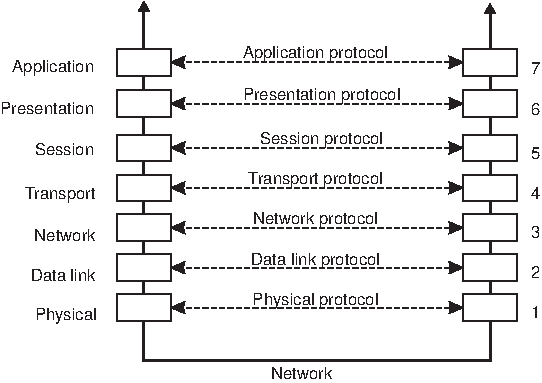
\includegraphics[scale=0.71]{04-01}
  \end{figure}

  \begin{block}{Desvantagens:}
    \begin{itemize}
    \item Funciona apenas com passagem de mensagens
    \item Frequentemente possuem funcionalidades desnecessárias
    \item Viola a transparência de acesso
    \end{itemize}
  \end{block}

\end{frame}

\begin{frame}
  \frametitle{Camadas de baixo nível}
  \begin{description}
  \item[Camada física:] contém a especificação e implementação dos bits em um quadro, e como são transmitidos entre o remetente e destinatário
  \item[Camada de enlace:] determina o envio de séries de bits em um quadro, permite detecção de erro e controle de fluxo
  \item[Camada de rede:] determina como pacotes são \alert{roteados} em uma rede de computadores
  \end{description}

  \begin{block}{Observação:}
    Em muitos sistemas distribuídos, a interface de mais baixo nível é a interface de rede.
  \end{block}

\end{frame}

\begin{frame}
  \frametitle{Camada de transporte}
  \begin{alertblock}{Importante:}
    A camada de transporte fornece as ferramentas de comunicação efetivamente utilizadas pela maioria dos sistemas distribuídos.
  \end{alertblock}

  \begin{block}{Protocolos padrões da Internet}
    \begin{description}
    \item[TCP:] orientada a conexão, confiável, comunicação orientada a fluxo de dados
    \item[UDP:] comunicação de datagramas não confiável (\textit{best-effort})
    \end{description}
  \end{block}

  \begin{alertblock}{Nota:}
    IP multicasting é normalmente considerado um serviço padrão (mas essa é uma hipótese perigosa)
  \end{alertblock}

\end{frame}

\begin{frame}
  \frametitle{Camada de middleware}
  \begin{block}{}
    Middleware foi inventado para prover serviços e protocolos
    \alert{frequentemente usados} que podem ser utilizados por várias
    aplicações \alert{diferentes}.
  \end{block}

  \begin{itemize}
  \item Um conjunto rico de \alert{protocolos de comunicação}
  \item \alert{(Des)empacotamento} [\textit{(un)marshaling}] de dados, necessários para a integração de sistemas
  \item \alert{Protocolos de gerenciamento de nomes}, para auxiliar o compartilhamento de recursos
  \item \alert{Protocolos de segurança} para comunicações seguras
  \item \alert{Mecanismos de escalabilidade}, tais como replicação e caching
  \end{itemize}

  \small
  \begin{alertblock}{Observação:}
    O que realmente sobra são protocolos específicos de aplicação.
  \end{alertblock}

\end{frame}

\begin{frame}
  \frametitle{Tipos de comunicação}

  \begin{figure}
    \centering
    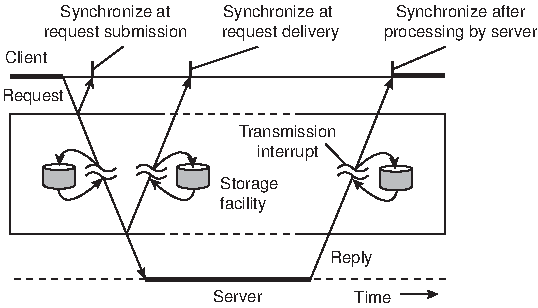
\includegraphics[scale=0.8]{04-04}
  \end{figure}

   \begin{overprint}

    \onslide<1>
    \begin{itemize}
    \item Comunicação \alert{transiente} vs. \alert{persistente}
    \item Comunicação \alert{assíncrona} vs. \alert{síncrona}
    \end{itemize}

    \onslide<2>
    \vspace{-1em}
    \begin{block}{Transiente vs. persistente}
      \begin{description}
      \item[Comunicação transiente:] remetente descarta a mensagem se ela não puder ser encaminhada para o destinatário
      \item[Comunicação persistente:] uma mensagem é guardada no remetente pelo tempo que for necessário, até ser entregue no destinatário
      \end{description}
    \end{block}

    \onslide<3>
    \begin{block}{Pontos de sincronização}
      \begin{itemize}
      \item No envio da requisição
      \item Na entrega da requisição
      \item Após o processamento da requisição
      \end{itemize}
    \end{block}
  \end{overprint}

\end{frame}

\begin{frame}
  \frametitle{Cliente/Servidor}

  Computação Cliente/Servidor geralmente é baseada em um modelo de \alert{comunicação transiente síncrona}:
  \begin{itemize}
  \item Cliente e servidor devem estar ativos no momento da comunicação
  \item Cliente envia uma requisição e bloqueia até que receba sua resposta
  \item Servidor essencialmente espera por requisições e as processa
  \end{itemize}

  \pause
  \begin{block}{Desvantagens de comunicação síncrona:}
    \begin{itemize}
    \item o cliente não pode fazer nenhum trabalho enquanto estiver esperando por uma resposta
    \item falhas precisam ser tratadas imediatamente (afinal, o cliente está esperando)
    \item o modelo pode não ser o mais apropriado (mail, news)
    \end{itemize}
  \end{block}

\end{frame}

\begin{frame}
  \frametitle{Trocas de mensagem}
  \begin{block}{Middleware orientado a mensagens}
    tem como objetivo prover \alert{comunicação persistente assíncrona}:
    \begin{itemize}
    \item Processos trocam mensagens entre si, as quais são armazenadas em uma fila
    \item O remetente não precisa esperar por uma resposta imediata, pode fazer outras coisas enquanto espera
    \item Middleware normalmente assegura tolerância a falhas
    \end{itemize}
  \end{block}
\end{frame}


\section{RPC --- Chamadas a procedimentos remotos}

\begin{frame}
  \frametitle{Chamadas a procedimentos remotos (RPC)}

  \begin{itemize}
  \item Funcionamento básico de RPCs
  \item Passagem de parâmetros
  \item Variações
  \end{itemize}

\end{frame}

\begin{frame}
  \frametitle{Funcionamento básico de RPC}
  \begin{itemize}
  \item Desenvolvedores estão familiarizados com o modelo de procedimentos
  \item Procedimentos bem projetados operam isoladamente (\textit{black box})
  \item Então não há  razão  para não executar esses procedimentos em máquinas separadas
  \end{itemize}

  \begin{columns}
    \begin{column}{0.5\textwidth}
      \begin{alertblock}{Conclusão}
        Comunicação entre o chamador \& chamado podem ser escondida com o uso de mecanismos de chamada a procedimentos.
      \end{alertblock}
    \end{column}
    \begin{column}{0.5\textwidth}
      \begin{figure}[centering]
        \centering
        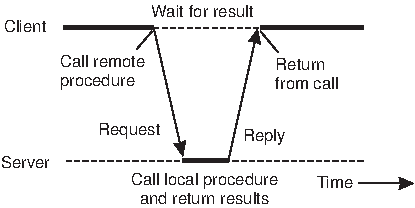
\includegraphics[width=\textwidth]{04-06}
      \end{figure}
    \end{column}
  \end{columns}

\end{frame}

\begin{frame}
  \frametitle{Funcionamento básico de RPC}

  \begin{figure}
    \centering
    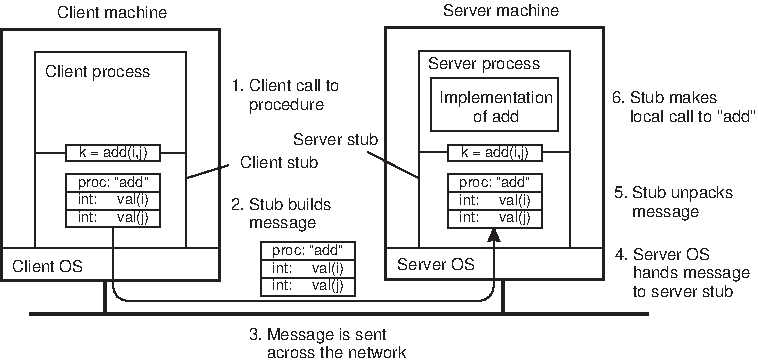
\includegraphics[scale=0.7]{04-07}
  \end{figure}

  \scriptsize
      \begin{tabular}{@{}ll}
        \begin{minipage}{0.45\textwidth}
          \begin{enumerate}%\setlength{\itemsep}{0pt}\zeroskip
          \item Procedimento no cliente chama o \textit{stub} do cliente
          \item \textit{Stub} constrói mensagem; chama o SO local
          \item SO envia msg. para o SO remoto
          \item SO remoto repassa mensagem para o \textit{stub}
          \item \textit{Stub} desempacota parâmetros e chama o servidor
          \end{enumerate}
        \end{minipage} &

        \begin{minipage}{0.45\textwidth}
          \begin{enumerate}
            %\setlength{\itemsep}{0pt}
            %\zeroskip
            \setcounter{enumi}{5}
          \item Servidor realiza chamada local e devolve resultado para o \textit{stub}
          \item \textit{Stub} constrói mensagem; chama SO
          \item SO envia mensagem para o SO do cliente
          \item SO do cliente repassa msg. para o \textit{stub}
          \item \textit{Stub} do cliente desempacota resultado e devolve para o cliente
          \end{enumerate}
        \end{minipage}
      \end{tabular}
\end{frame}

\begin{frame}
  \frametitle{RPC: passagem de parâmetros}

  \begin{block}{Empacotamento de parâmetros} há mais do que apenas colocá-los nas mensagens:

    \begin{itemize}
    \item As máquinas cliente e servidor podem ter \alert{representação de dados diferentes} (ex: ordem dos bytes)
    \item Empacotar um parâmetro significa \alert{transformar um valor em uma sequência de bytes}
    \item Cliente e servidor precisam concordar com a mesma regra de codificação (\textit{encoding}):
      \begin{itemize}
      \item Como os \alert{valores dos dados básicos} (inteiros, números em ponto flutuante, caracteres) são representados?
      \item Como os \alert{valores de dados complexos} (vetores, \textit{unions}) são representados?
      \end{itemize}

      \item Cliente e servidor precisam \alert{interpretar corretamente as mensagens}, transformando seus valores usando representações dependentes da máquina
    \end{itemize}
  \end{block}
\end{frame}

\begin{frame}
  \frametitle{RPC: passagem de parâmetros}
  \begin{block}{Algumas suposições:}
    \begin{itemize}
    \item semântica de \alert{copy in/copy out}: enquanto um procedimento é executado, nada pode ser assumido sobre os valores dos parâmetros
    \item \alert{Todos} os dados são passado apenas por parâmetro. Exclui passagem de \emph{referências para dados (globais)}.
    \end{itemize}
  \end{block}

  \pause
  \begin{alertblock}{Conclusão}
    Não é possível assumir transparência total de acesso.
  \end{alertblock}

  % \pause
  % \begin{block}{Um mecanismo de referências remotas melhoraram a transparência de acesso:}
  %   \begin{itemize}
  %   \item Referências remotas oferecem \alert{acesso unificado} a dados remotos
  %   \item Referências remotas podem ser \alert{passados como parâmetro} em RPCs
  %   \end{itemize}
  % \end{block}
\end{frame}

\begin{frame}
  \frametitle{RPC assíncrono}
  \begin{block}{Ideia geral}
    Tentar se livrar do comportamento estrito de requisição--resposta, mas permitir que o cliente continue sem esperar por uma resposta do servidor.
  \end{block}

  \begin{figure}
    \centering
    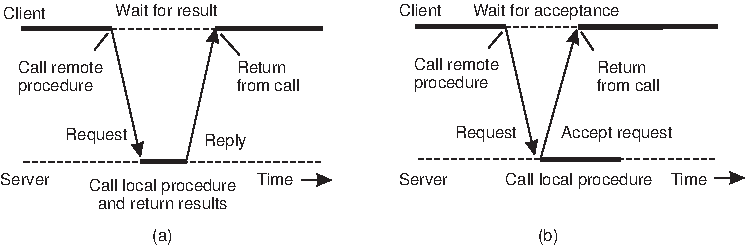
\includegraphics[width=\textwidth]{04-10}
  \end{figure}

\end{frame}

\begin{frame}
  \frametitle{RPC síncrono diferido}
  \begin{figure}
    \centering
    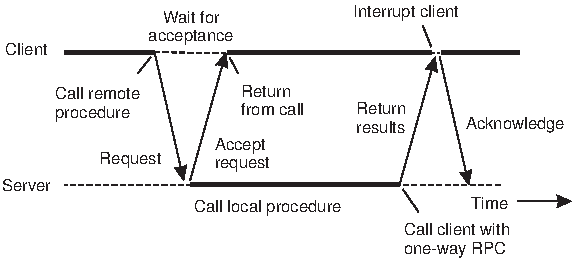
\includegraphics[width=\textwidth]{04-11}
  \end{figure}

  \begin{block}{Variação}
    Cliente pode também realizar uma consulta (\textit{poll}) (bloqueante ou não) para verificar se os resultados estão prontos.
  \end{block}

\end{frame}

\begin{frame}
  \frametitle{RPC na prática}
  \begin{figure}
    \centering
    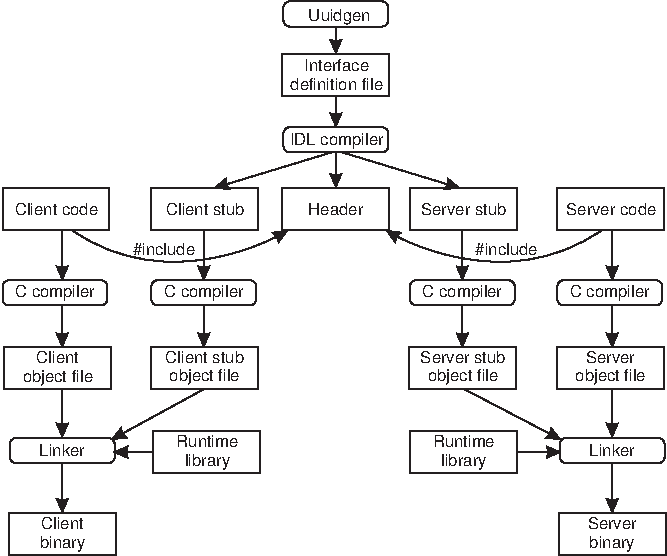
\includegraphics[scale=0.85]{04-12}
  \end{figure}

% %%     Let the developer concentrate on only the client- and server-specific code; let the RPC system (generators
% %%     and libraries) do the rest.

\end{frame}

\begin{frame}
  \frametitle{Vinculação cliente--servidor (DCE)}

  \begin{block}{Problemas}
    (1)~Cliente precisa localizar a máquina com o servidor e,\\
    (2)~precisa localizar o servidor.
  \end{block}

  \begin{figure}
    \centering
    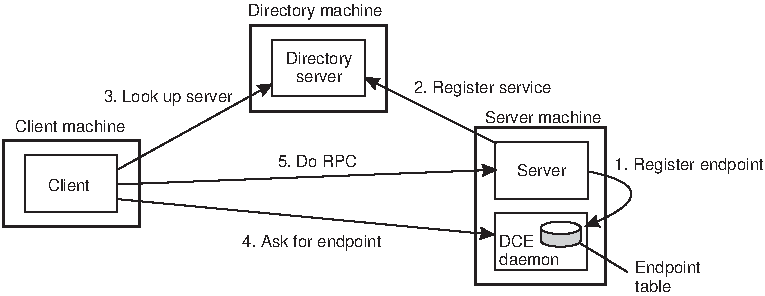
\includegraphics[width=\textwidth]{04-13}
  \end{figure}

\end{frame}

\section{Comunicação orientada a mensagens}

\begin{frame}
  \frametitle{Comunicação orientada a mensagens}
  \begin{itemize}
  \item Mensagens transientes
  \item Sistema de enfileiramento de mensagens
  \item \textit{Message brokers}
  \item Exemplo: IBM Websphere
  \end{itemize}
\end{frame}

\begin{frame}
  \frametitle{Mensagens transientes: sockets}
  \begin{exampleblock}{Berkeley socket interface}
    \begin{center}
      \small
      \renewcommand{\arraystretch}{1.1}
      \begin{tabular}{|>{\texttt}l|l|}\hline
        \texttt{SOCKET}  & Cria um novo ponto de comunicação \\ \hline
        \texttt{BIND}    & Especifica um endereço local ao socket \\ \hline
        \texttt{LISTEN}  & Anuncia a vontade de receber $N$ conexões \\ \hline
        \texttt{ACCEPT}  & Bloqueia até receber um pedido de estabelecimento de conexão \\ \hline
        \texttt{CONNECT} & Tenta estabelecer uma conexão \\ \hline
        \texttt{SEND}    & Envia dados por uma conexão \\ \hline
        \texttt{RECEIVE} & Recebe dados por uma conexão \\ \hline
        \texttt{CLOSE}   & Libera a conexão \\ \hline
      \end{tabular}
    \end{center}
  \end{exampleblock}
\end{frame}

\begin{frame}
  \frametitle{Mensagens transientes: sockets}
  \begin{figure}
    \centering
    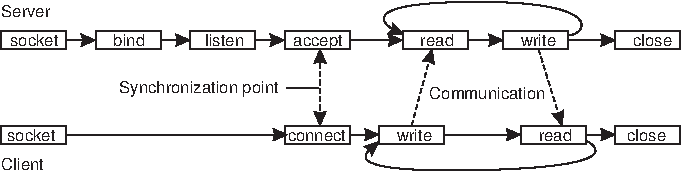
\includegraphics[width=\textwidth]{04-15}
  \end{figure}
\end{frame}

\begin{frame}[fragile]
  \frametitle{Sockets: código em Python}
\begin{minted}{python}
import socket
HOST = socket.gethostname()          # e.g. 'localhost'
PORT = SERVERPORT                    # e.g.  80
s = socket.socket(socket.AF_INET, socket.SOCK_STREAM)
s.bind((HOST, PORT))
s.listen(N)         # listen to max N queued connection
conn, addr = s.accept()      # new socket + addr client
while 1: # forever
  data = conn.recv(1024)
  if not data: break
  conn.send(data)
conn.close()
\end{minted}
\end{frame}

\begin{frame}
  \frametitle{Middleware orientado a mensagens}
  \begin{block}{Ideia geral}
    Comunicação assíncrona e persistente graças ao uso de \alert{filas} pelo middleware. Filas correspondem a buffers em servidores de comunicação.
  \end{block}

  \begin{center}
    \small
    \renewcommand{\arraystretch}{1.1}
    \begin{tabular}{|>{\texttt}l|p{8cm}|}\hline
      \texttt{PUT}    & Adiciona uma mensagem à fila especificada \\ \hline
      \texttt{GET}    & Bloqueia até que a fila especificada tenha alguma mensagem e remove a primeira mensagem \\ \hline
      \texttt{POLL}   & Verifica se a fila especificada tem alguma mensagem e remove a primeira. Nunca bloqueia \\ \hline
      \texttt{NOTIFY} & Instala um tratador para ser chamado sempre que uma mensagem for inserida em uma dada fila \\ \hline
    \end{tabular}
  \end{center}

\end{frame}

\begin{frame}
  \frametitle{Message broker}
  \begin{block}{Observação:}
    Sistemas de filas de mensagens assumem um \alert{protocolo comum de troca de mensagens}: todas as aplicações usam o mesmo formato de mensagem (i.e., estrutura e representação de dados)
  \end{block}

  \begin{block}{Message broker}
    Componente centralizado que lida com a heterogeneidade das
    aplicações:
    \begin{itemize}
    \item transforma as mensagens recebidas para o formato apropriado
    \item frequentemente funciona como um \alert{application gateway}
    \item podem rotear com \alert{base no conteúdo} $\Rightarrow$ \alert{Enterprise Application Integration}
    \end{itemize}
  \end{block}

\end{frame}

\begin{frame}
  \frametitle{Message broker}
  \begin{figure}
    \centering
    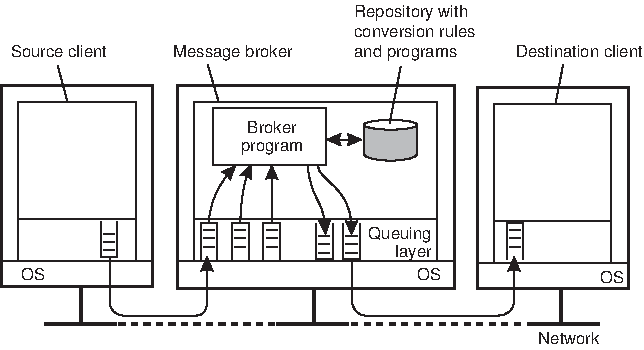
\includegraphics[width=\textwidth]{04-21}
  \end{figure}
\end{frame}

% termos em pt-br em http://www.ibm.com/developerworks/br/local/websphere/mq_conceitos_melhores_praticas/index1.html
\begin{frame}
  \frametitle{IBM WebSphere  Message Queue (MQ)}

  \begin{itemize}
  \item \alert{Mensagens específicas da aplicação} são colocadas e removidas de \alert{filas}
  \item As filas são controladas por um \alert{gerenciador de filas}
  \item Processos podem colocar mensagens apenas em filas locais, ou usando um mecanismo de RPC
  \end{itemize}

\end{frame}


\begin{frame}
  \frametitle{IBM WebSphere MQ}

  \begin{block}{Transferência de mensagens}
    \begin{itemize}
    \item Mensagens são transferidas entre filas
    \item Mensagens transferidas entre filas em diferentes processos requerem um \alert{canal}
    \item Em cada ponta do canal existe um \alert{agente de canal}, responsável por:
      \begin{itemize}
      \item configurar canais usando ferramentas de rede de baixo nível (ex: TCP/IP)
      \item (Des)empacotar mensagens de/para pacotes da camada de transporte
      \item Enviar/receber pacotes
      \end{itemize}
    \end{itemize}
  \end{block}

\end{frame}

\begin{frame}
  \frametitle{IBM WebSphere MQ}

  \begin{figure}
    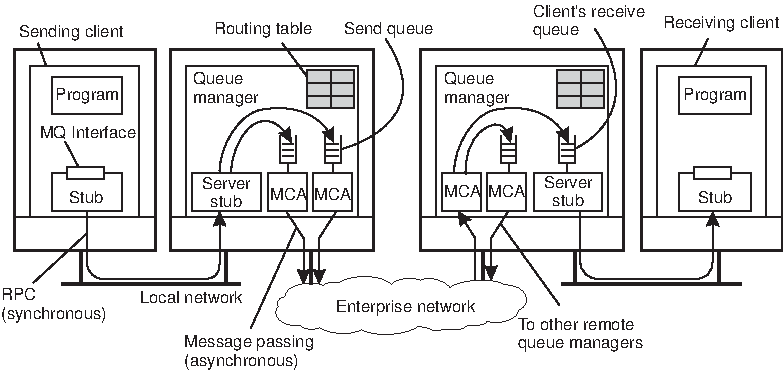
\includegraphics[width=\textwidth]{04-22}
  \end{figure}

  \begin{itemize}
  \item Canais são unidirecionais
  \item Agentes de canais são automaticamente iniciados quando uma mensagem chega
  \item Pode-se criar redes de gerenciadores de filas
  \item Rotas são configuradas manualmente (pelo admin do sistema)
  \end{itemize}

\end{frame}

\begin{frame}
  \frametitle{IBM WebSphere MQ}

  \begin{block}{Roteamento}
    O uso de \alert{nomes lógicos}, combinados com resolução de nomes para filas locais, permitem que uma mensagem seja colocada em uma \alert{fila remota}.
  \end{block}

  \begin{figure}
    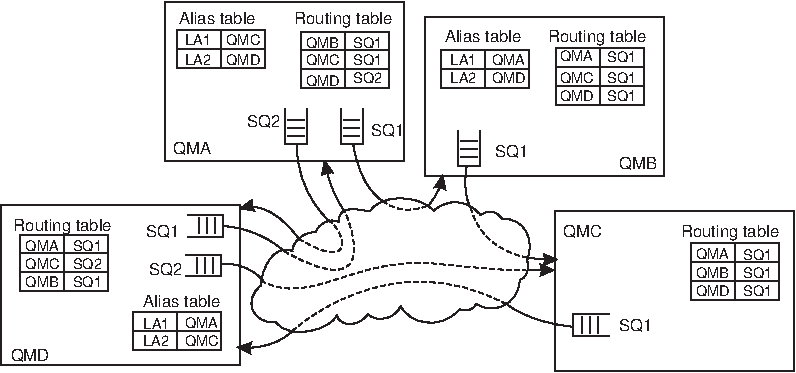
\includegraphics[width=\textwidth]{04-24}
  \end{figure}

\end{frame}


\end{document}
